%\newpage
\section{Обработка результатов измерений}
\subsection{Результаты измерений}
Приведем графики полученных спектров (рис. \ref{full_45}--\ref{full_65}). В день опытов атмосферное давление было равно $p_0 = 750$ торр. По полученным данным проведем идентификацию наблюдаемых полос (табл. \ref{tab:polosi}).
\begin{figure}[H]
	\begin{minipage}{0.45\linewidth}
		\centering
		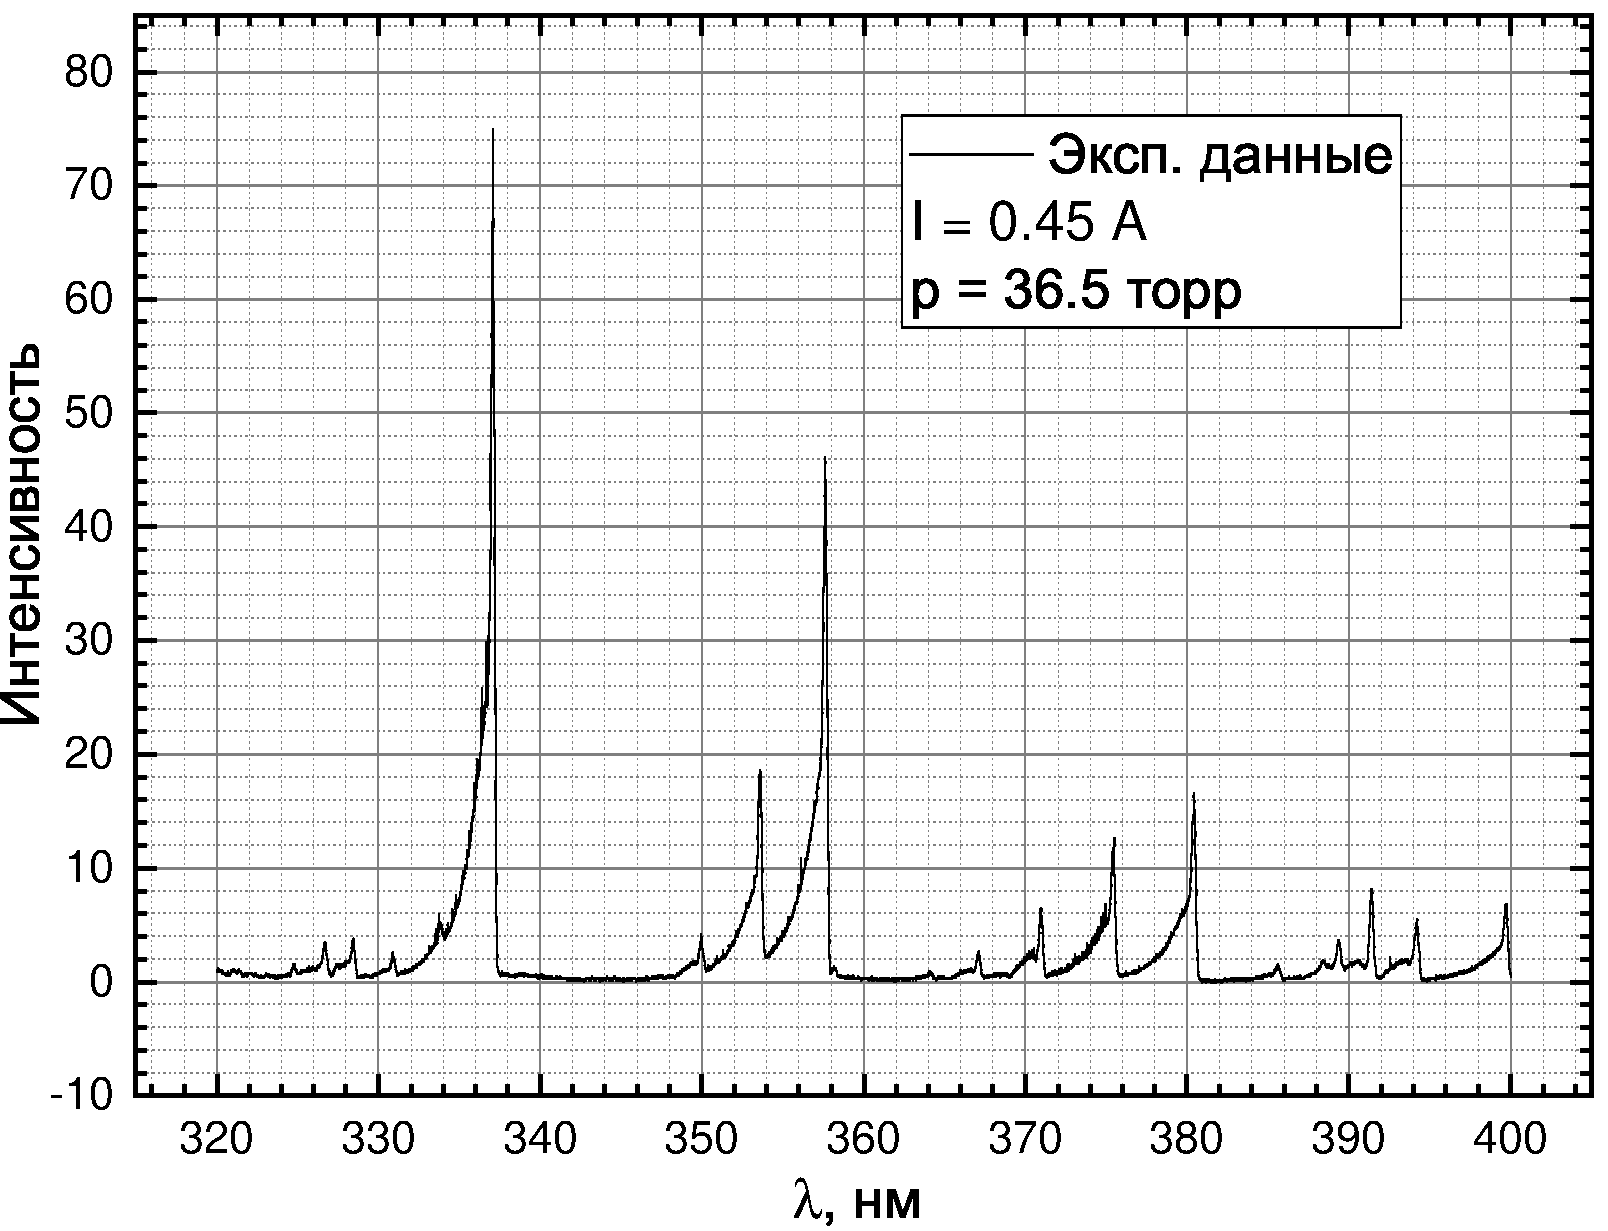
\includegraphics[width=\linewidth]{data/graph_I=0,45}
		\caption{Спектр при $I= 0.45$ А, $P$= 36.5 торр}
		\label{full_45}
	\end{minipage} 
	\hfill
	\begin{minipage}[H]{0.45\linewidth}
		\centering
		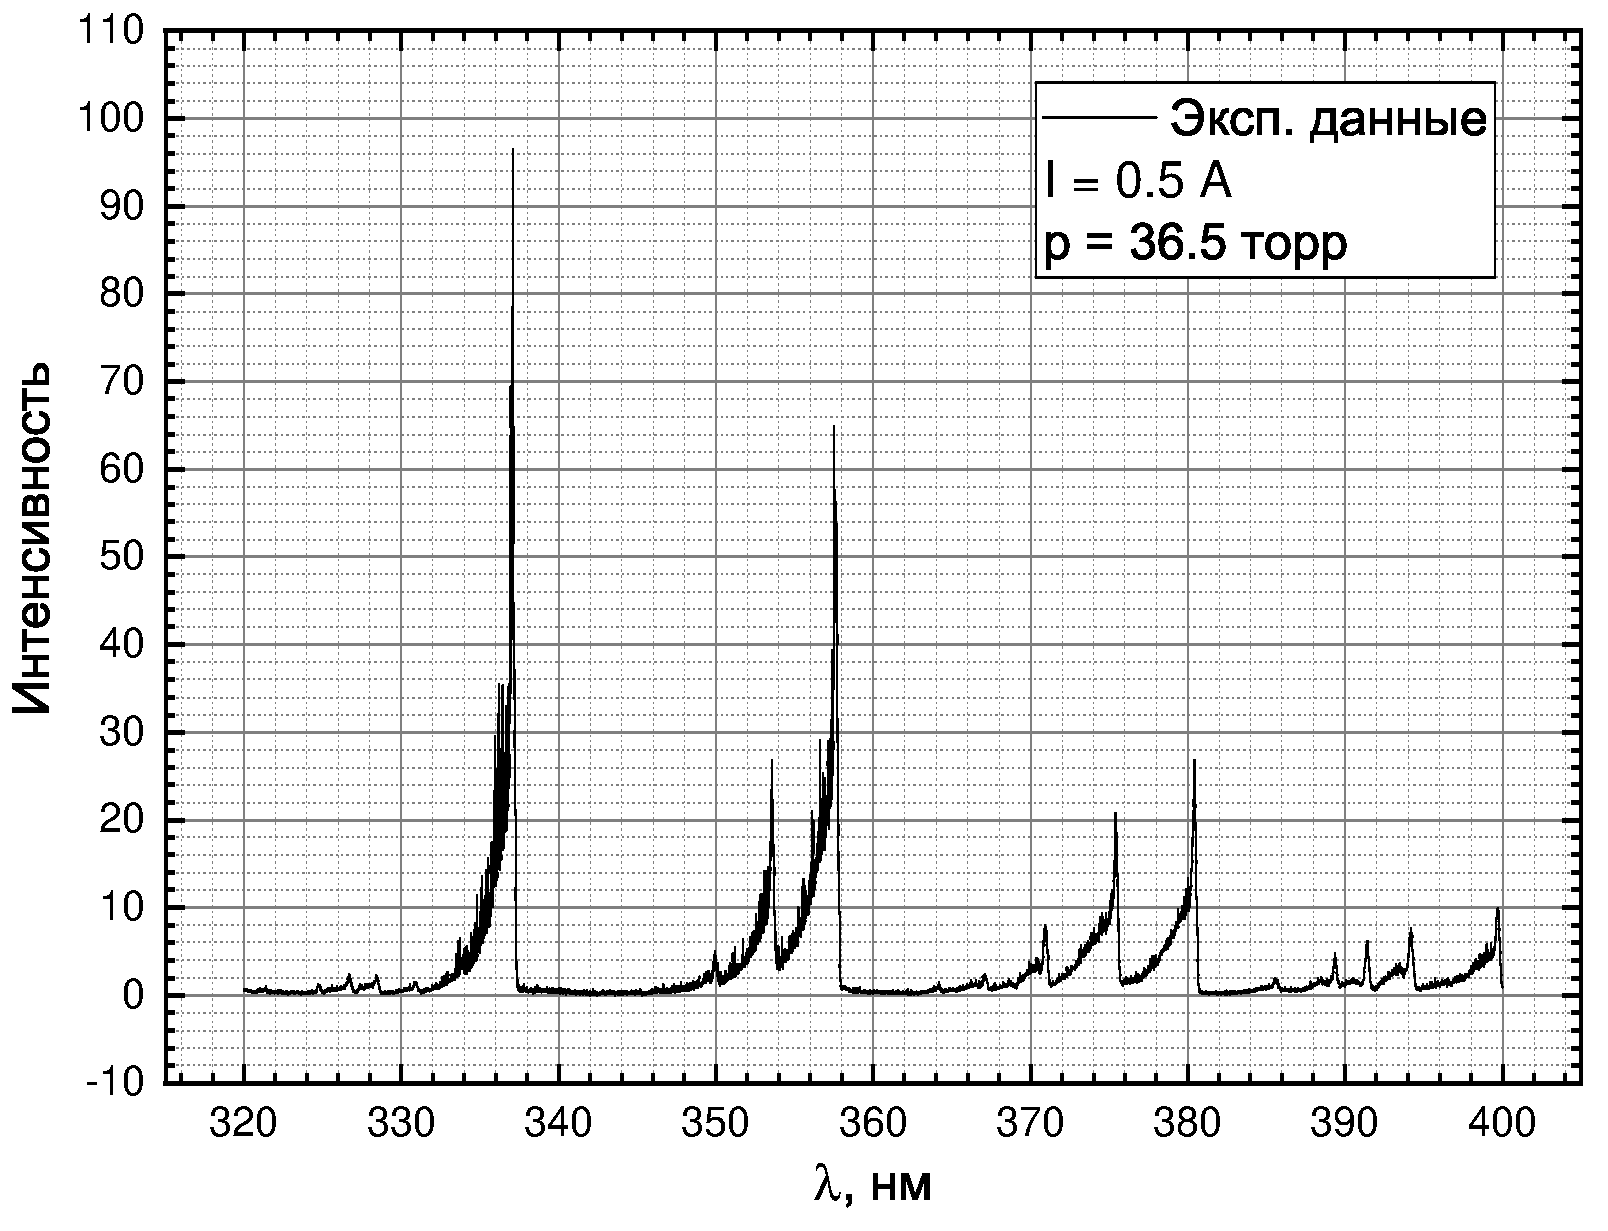
\includegraphics[width=\linewidth]{data/graph_I=0,50}
		\caption{Спектр при $I= 0.50 $ А, $P$= 36.5 торр}
		\label{full_50}
	\end{minipage}
	\begin{minipage}{0.45\linewidth}
		\centering
		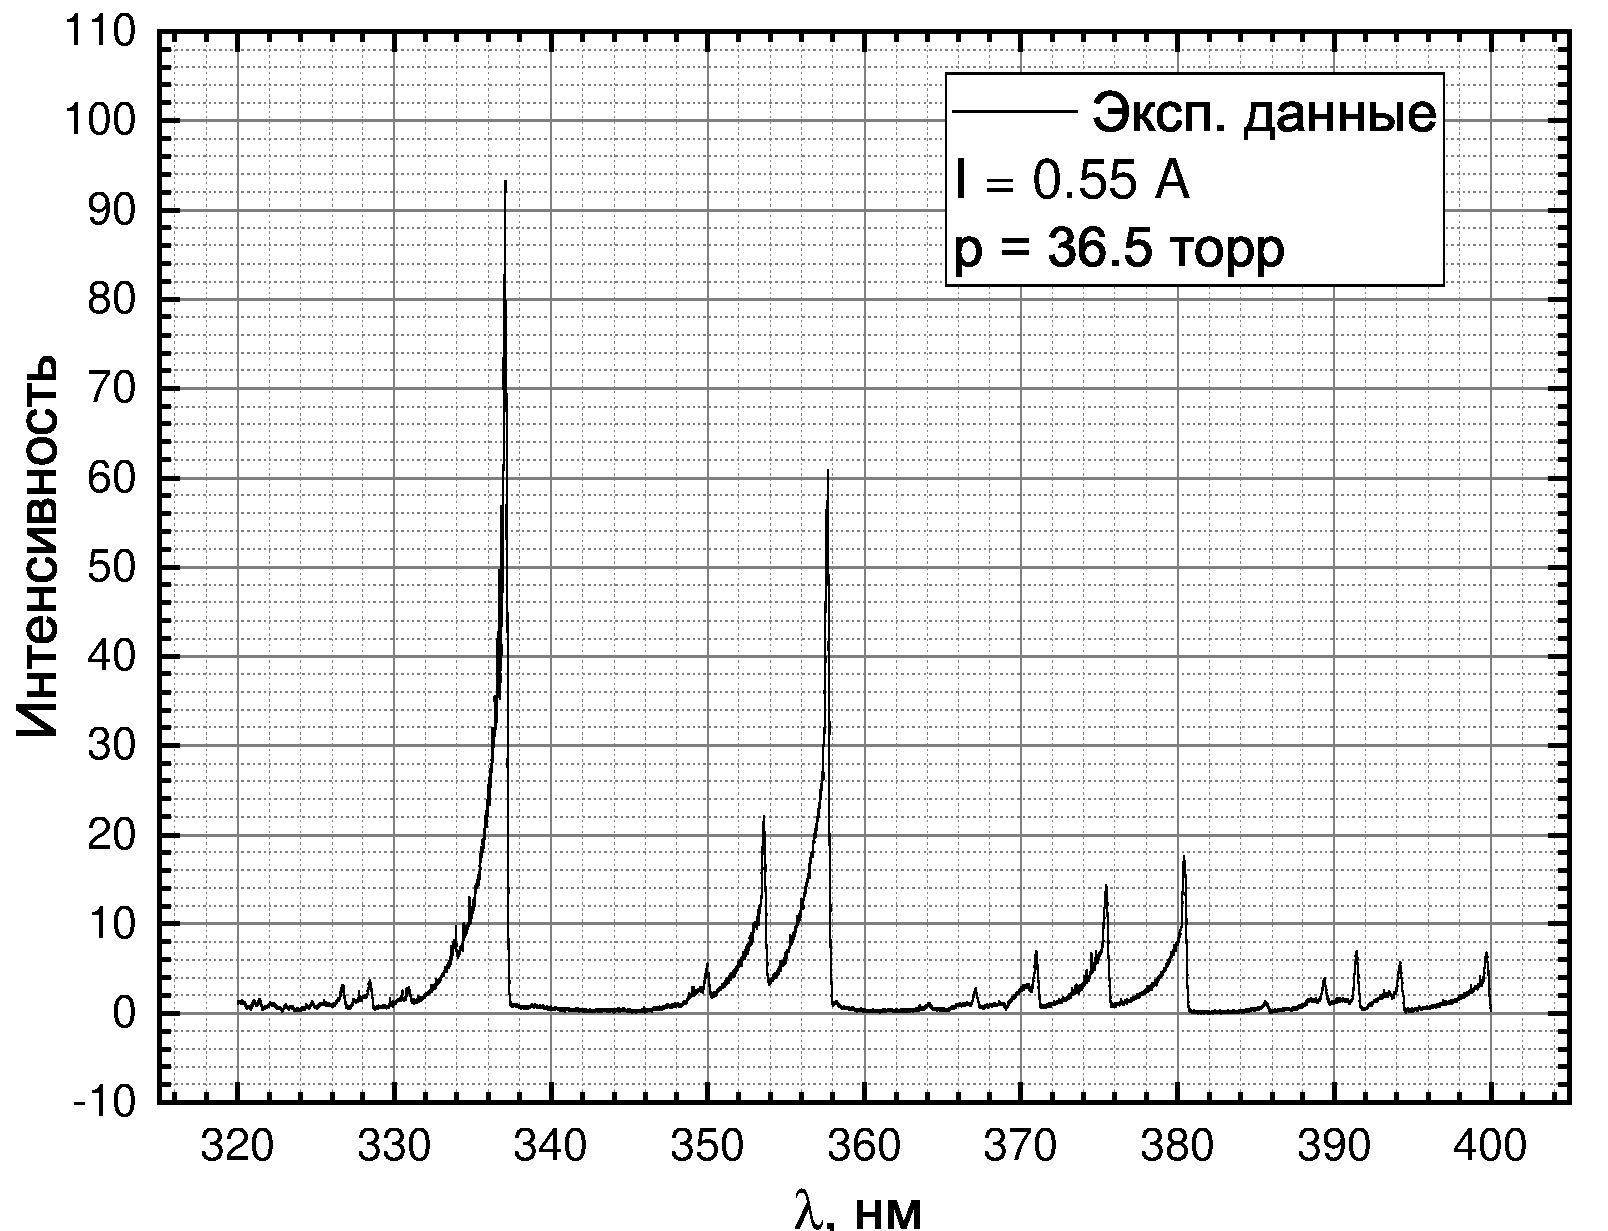
\includegraphics[width=\linewidth]{data/graph_I=0,55}
		\caption{Спектр при $I= 0.55 $ А, $P$= 36.5 торр}
		\label{full_55}	
	\end{minipage} 
	\hfill
	\begin{minipage}[H]{0.45\linewidth}
		\centering
		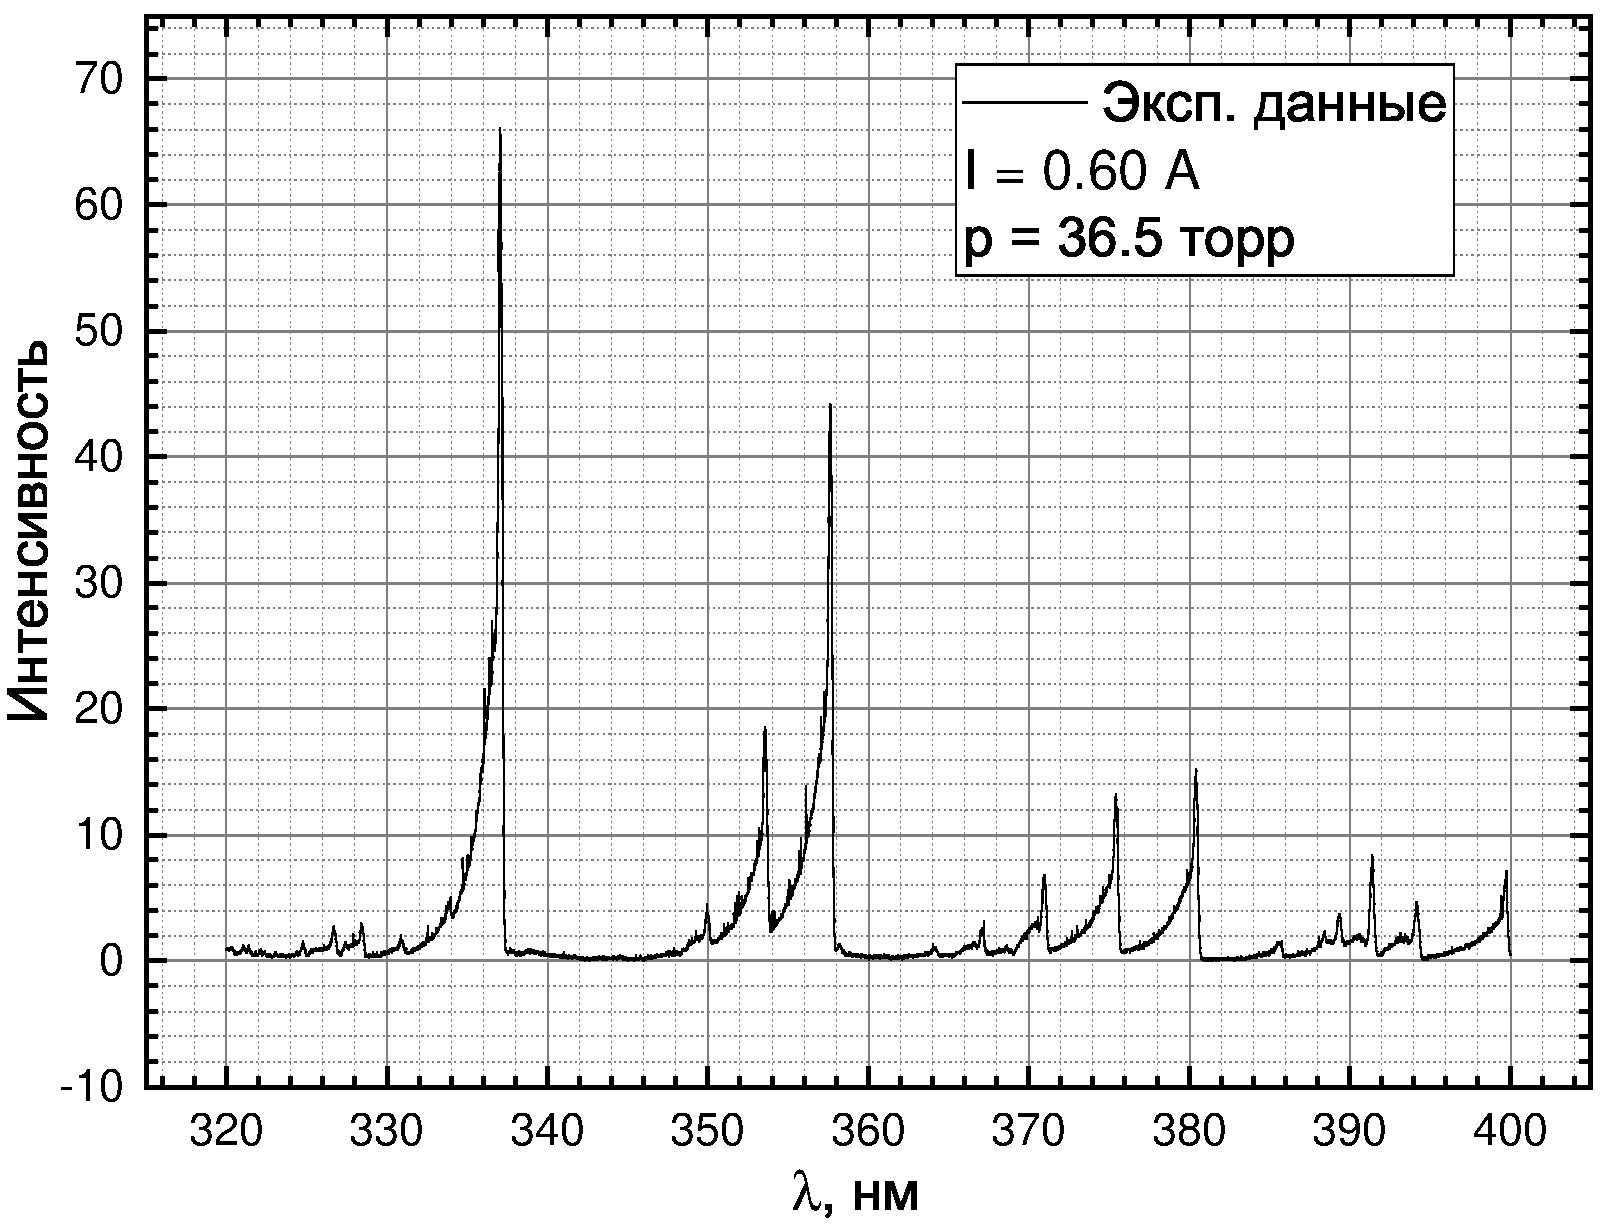
\includegraphics[width=\linewidth]{data/graph_I=0,60}
		\caption{Спектр при $I= 0.60 $ А, $P$= 36.5 торр}
		\label{full_60}
	\end{minipage}
	\begin{minipage}{0.45\linewidth}
		\centering
		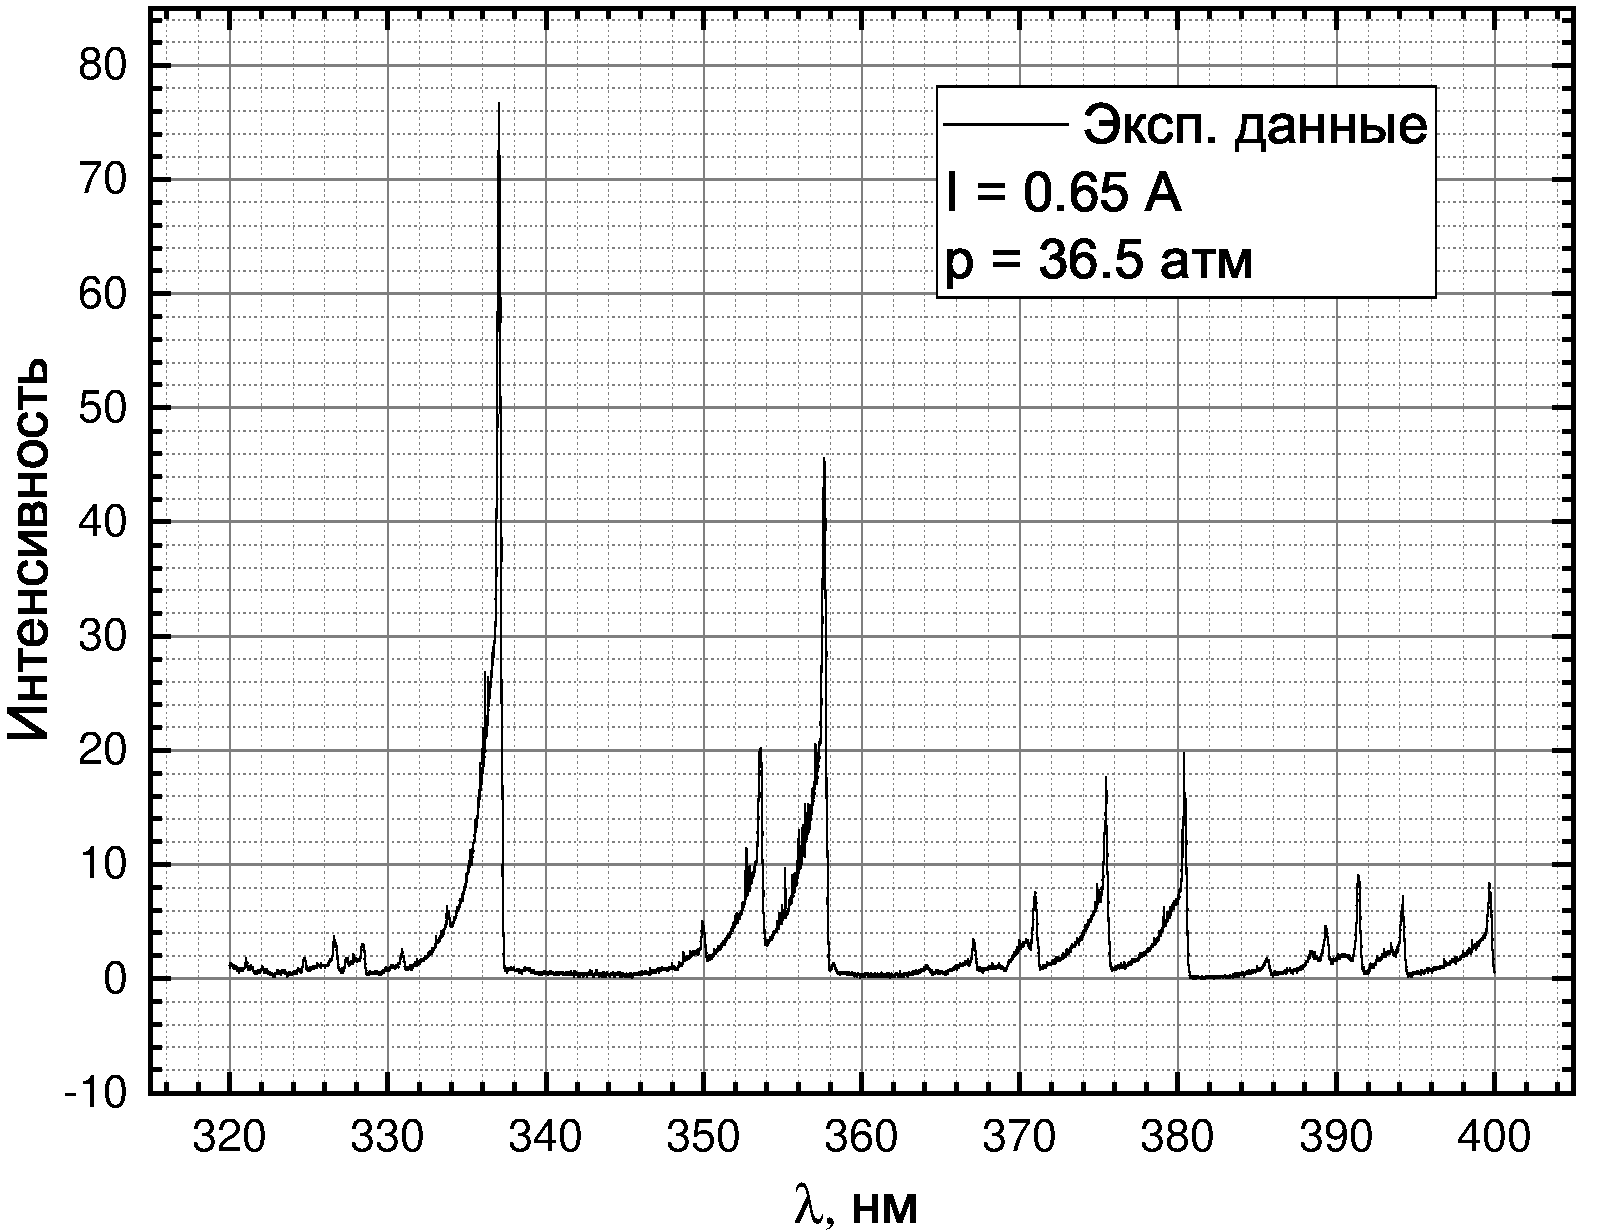
\includegraphics[width=\linewidth]{data/graph_I=0,65}
		\caption{Спектр при $I= 0.65 $ А, $P$= 36.5 торр}	
		\label{full_65}
	\end{minipage} 
	\hfill
\end{figure}

 % Table generated by Excel2LaTeX from sheet 'Лист1'
\begin{table}[H]
	\centering
	\caption{Соотнесение полос}
	\begin{tabular}{ | l | l | l | l | l | l | }
	\hline
	$I$, A & $\lambda$, нм & переход & $I$, A & $\lambda$, нм & переход \\
	\hline
	\hline
	0.65 & 337.03 & $0 \rightarrow 0$ & 0.60 & 337.06 & $0 \rightarrow 0$ \\ \hline
	0.65 & 357.61 & $0 \rightarrow 1$ & 0.60 & 357.64 & $0 \rightarrow 1$ \\ \hline
	0.65 & 353.60 & $1 \rightarrow 2$ & 0.60 & 353.55 &$ 1 \rightarrow 2$ \\ \hline
	0.65 & 349.92 & $2 \rightarrow 3$ & 0.60 & 349.93 & $2 \rightarrow 3$ \\ \hline
	0.65 & 380.37 & $0 \rightarrow 2$ & 0.60 & 380.42 & $0 \rightarrow 2$ \\ \hline
	0.65 & 375.44 & $1 \rightarrow 3$ & 0.60 & 375.42 & $1 \rightarrow 3$ \\ \hline
	0.65 & 370.97 & $2 \rightarrow 4$ & 0.60 & 370.98 & $2 \rightarrow 4$ \\ \hline
	0.65 & 367.06 & $3 \rightarrow 5$ & 0.60 & 367.19 & $3 \rightarrow 5$ \\ \hline
	\end{tabular}
	\label{tab:polosi}%
\end{table}%

\subsection{Вычисление вращательной температуры}
Для вычисления вращательной температуры выберем участок неразрешенной
вращательной структуры и прологарифмируем его. По наклону прямой зависимости $\lg I=f(\lambda)$ , используя рассчитанную
зависимость тангенса угла наклона от значения вращательной температуры, определим значение вращательной температуры в центральной части разряда. Результаты занесем в таблицу \ref{tab:T_rot}.

\begin{table}[H]
	\centering
	\caption{Расчет вращательной температуры по угловому коэффициенту}
	\begin{tabular}{|c|c|}
		\hline 
		$I$, A & $T_\text{rot}$, K \\ 
		\hline 
		0.45 & 1000 \\ 
		\hline 
		0.50 & 1382 \\ 
		\hline 
		0.55 & 1210 \\ 
		\hline 
		0.6 & 1209 \\ 
		\hline 
		0.65 & 1234 \\ 
		\hline 
	\end{tabular} 
	\label{tab:T_rot}
\end{table}

\begin{figure}[H]
	\begin{minipage}{0.45\linewidth}
		\centering
		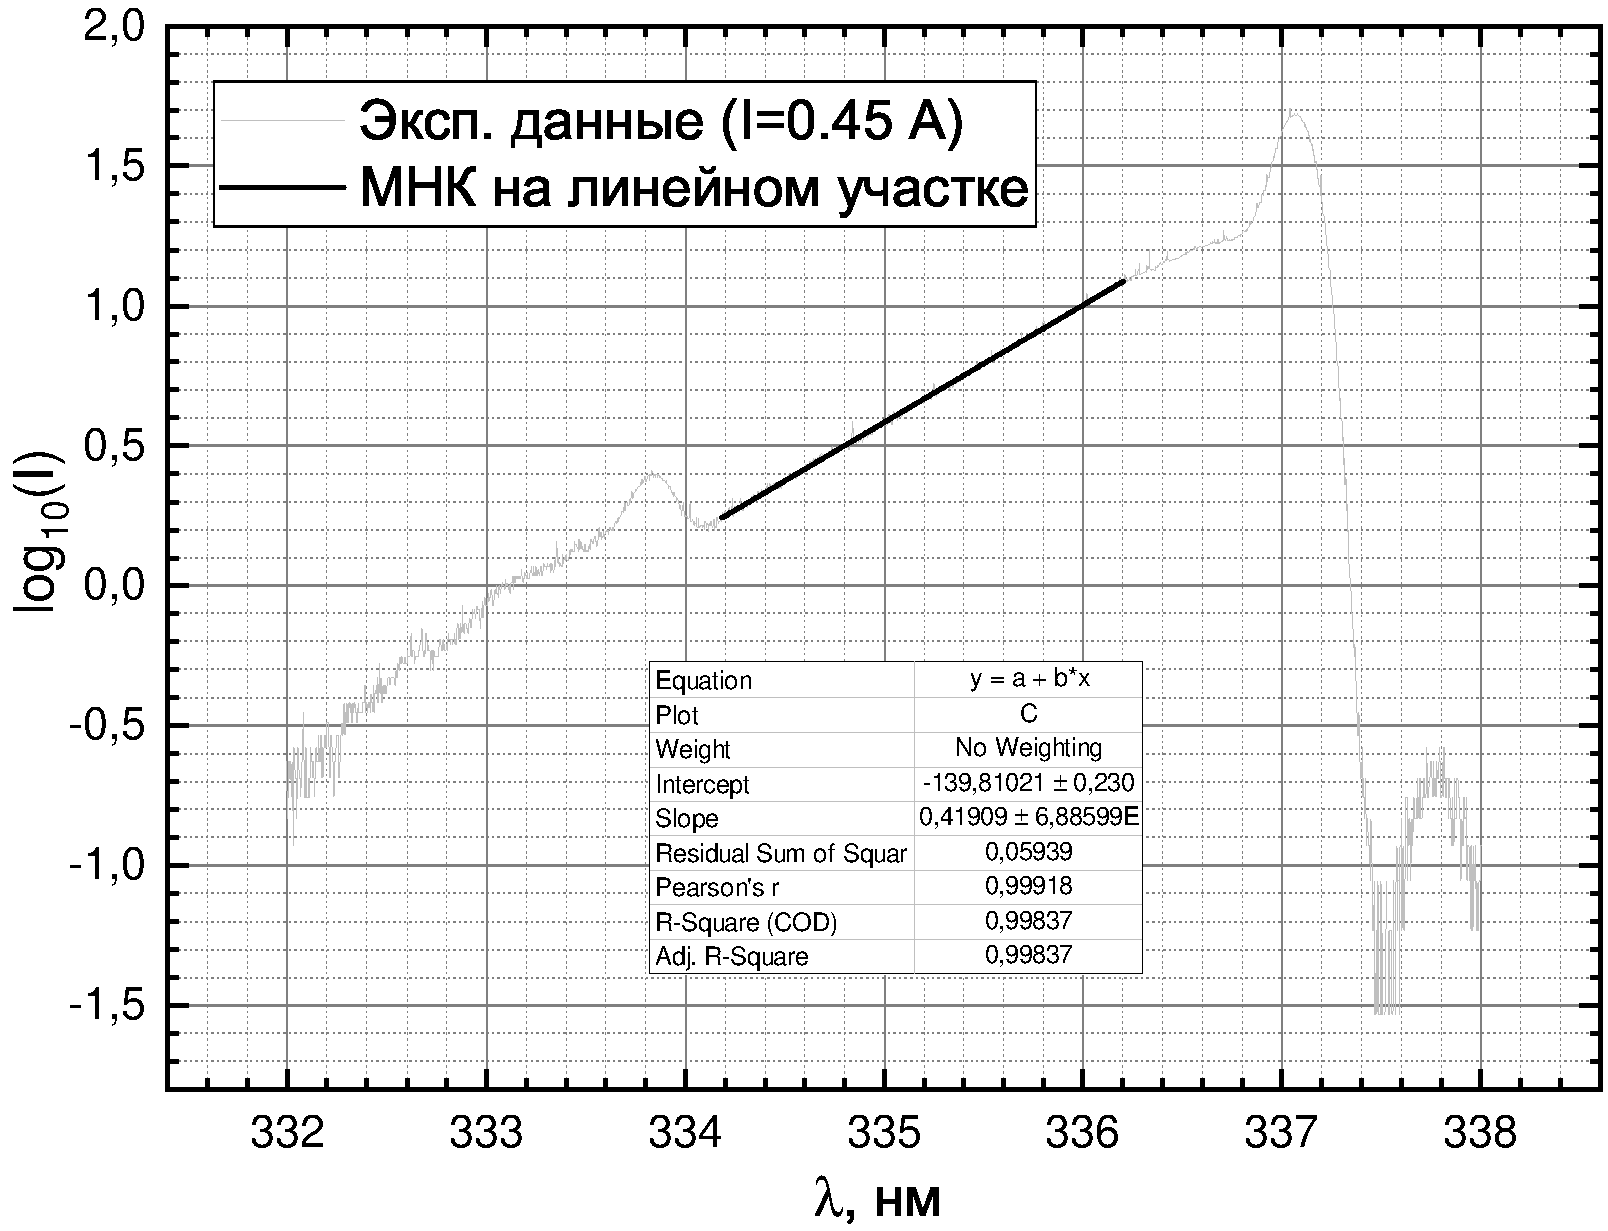
\includegraphics[width=\linewidth]{data/graph_I=0,45_polosa}
		\caption{Спектр при $I= 0.45$ А, $P$= 36.5 торр}
		\label{polosa_45}
	\end{minipage} 
	\hfill
	\begin{minipage}[H]{0.45\linewidth}
		\centering
		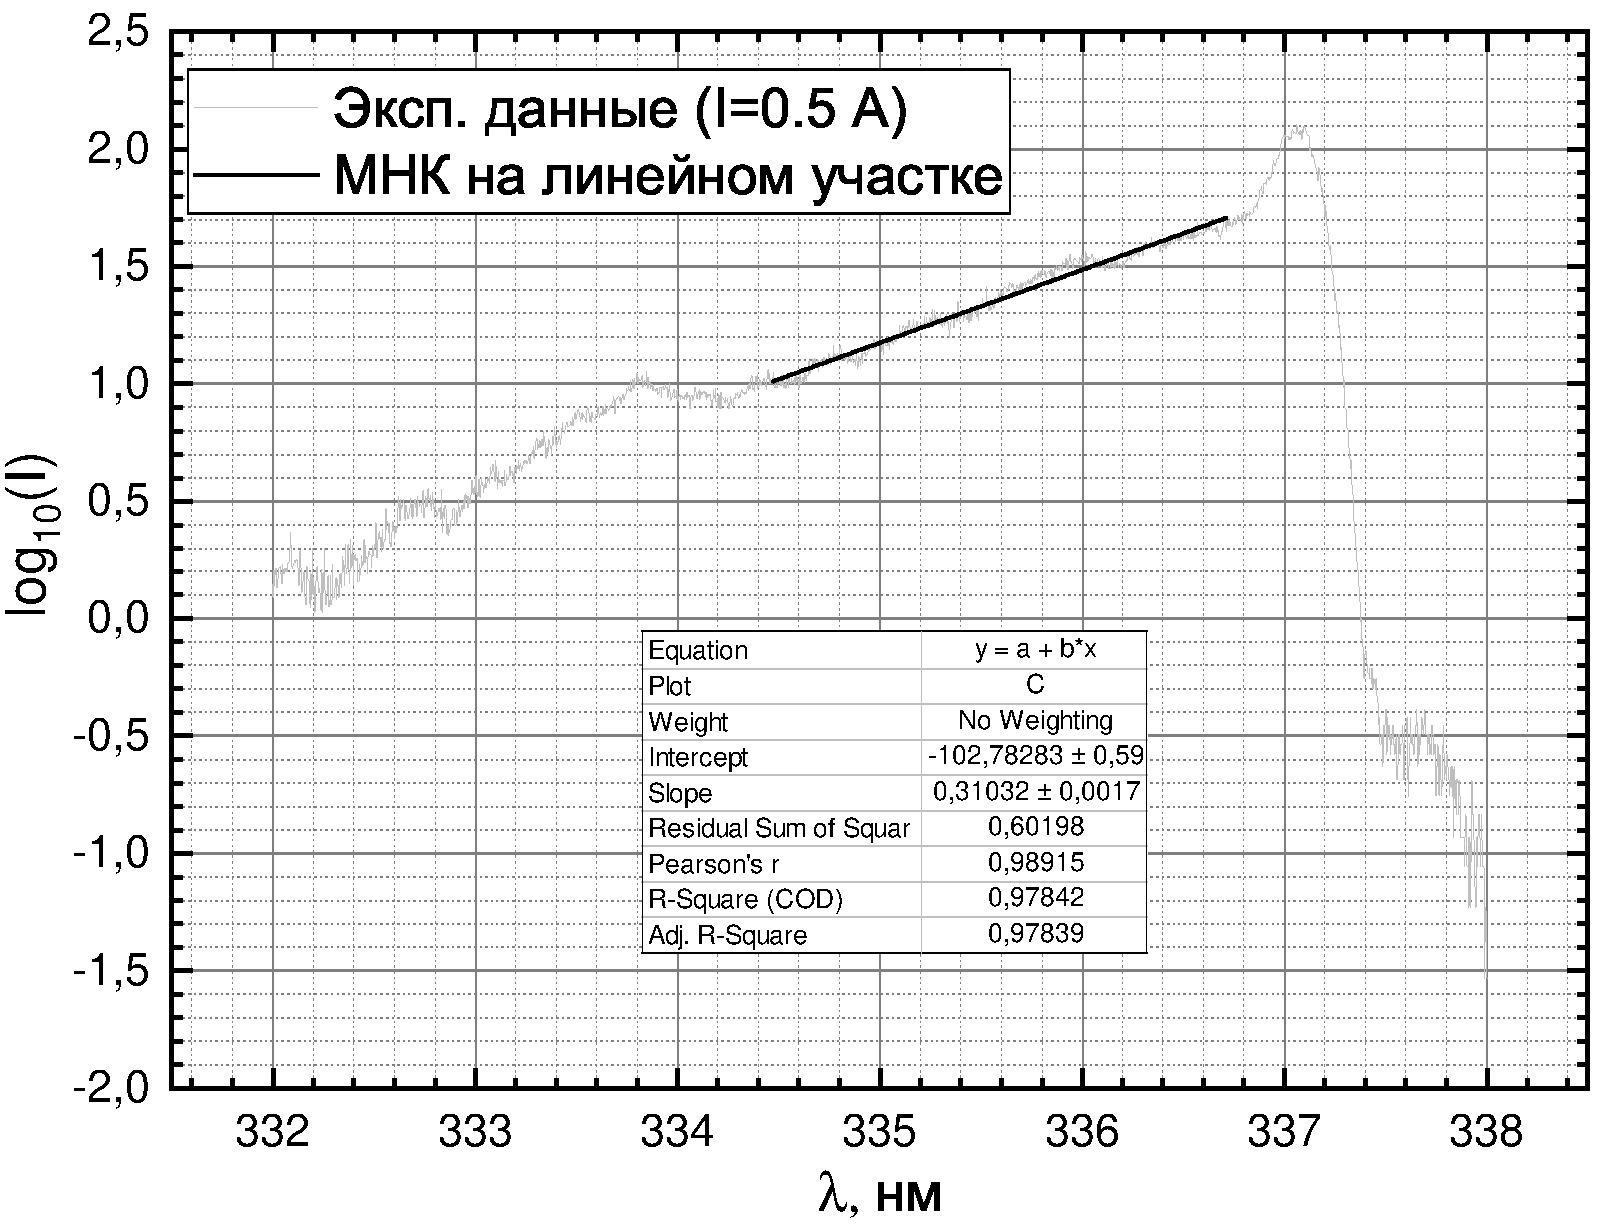
\includegraphics[width=\linewidth]{data/graph_I=0,50_polosa}
		\caption{Спектр при $I= 0.50 $ А, $P$= 36.5 торр}
		\label{polosa_50}
	\end{minipage}
	\begin{minipage}{0.45\linewidth}
		\centering
		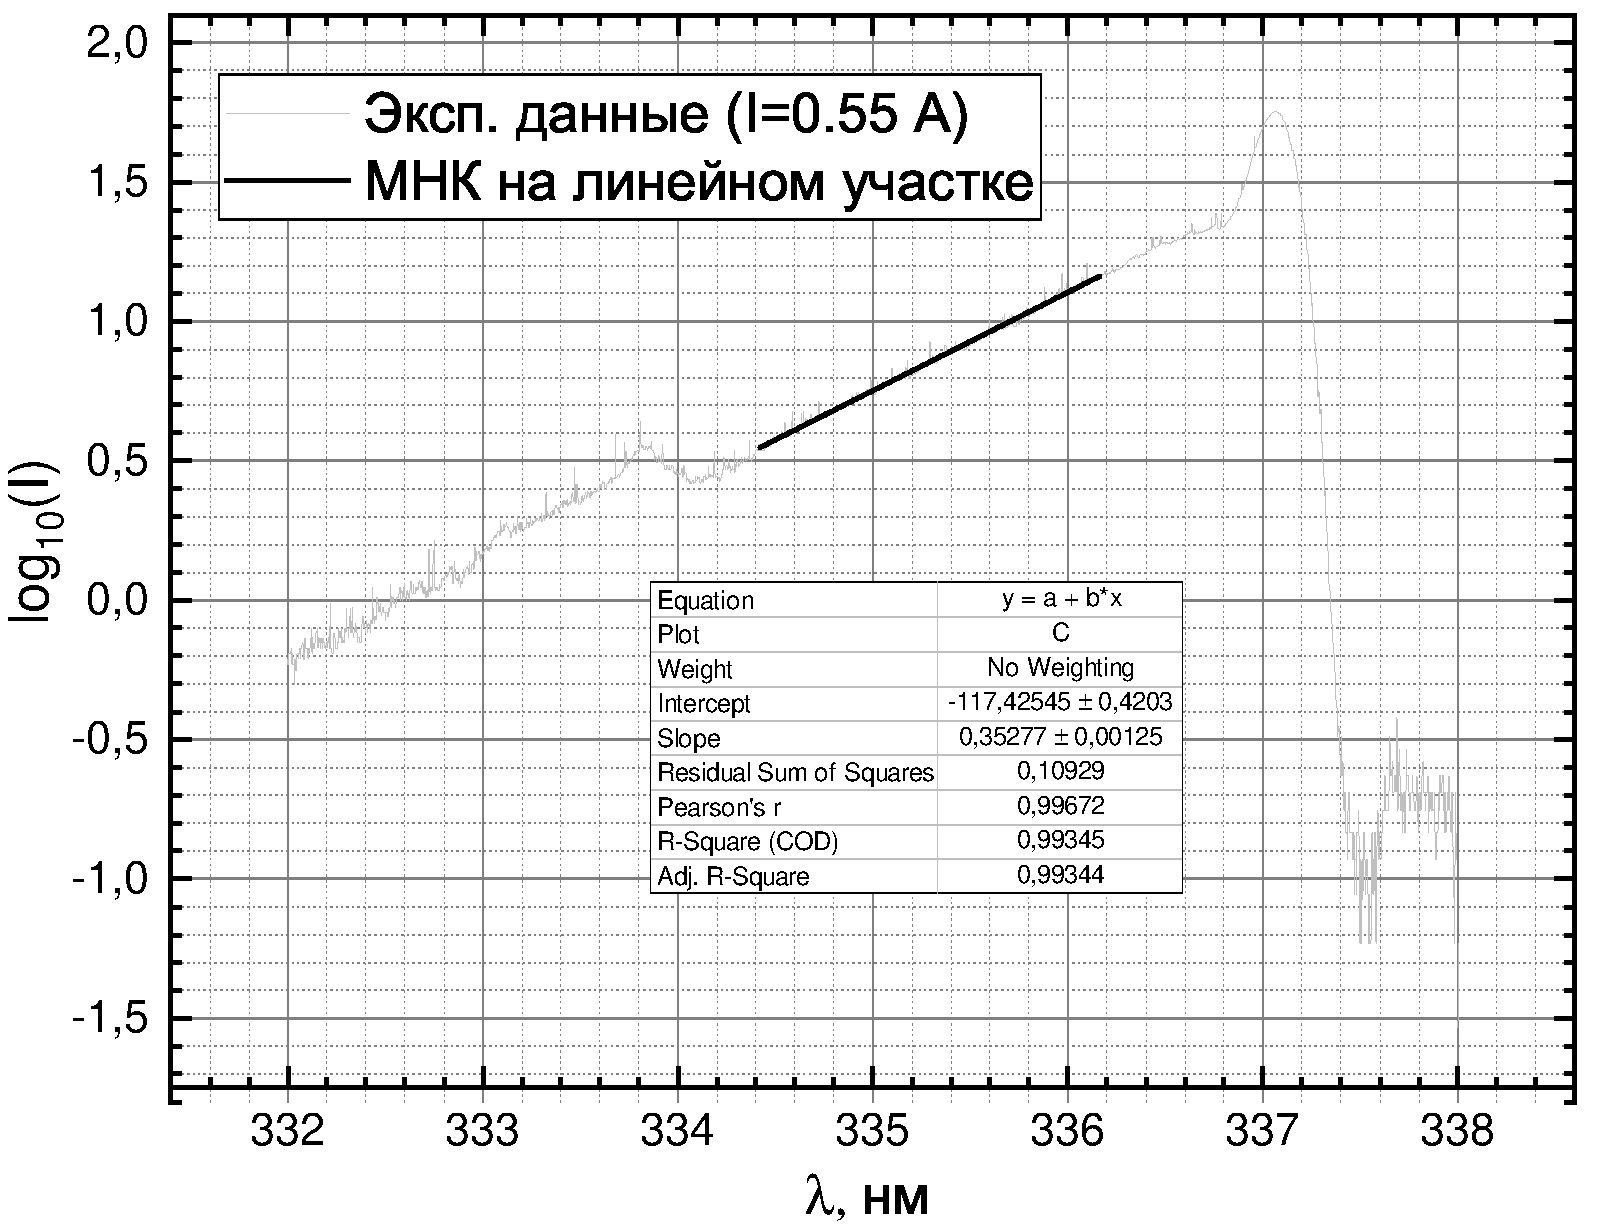
\includegraphics[width=\linewidth]{data/graph_I=0,55_polosa}
		\caption{Спектр при $I= 0.55 $ А, $P$= 36.5 торр}
		\label{polosa_55}	
	\end{minipage} 
	\hfill
	\begin{minipage}[H]{0.45\linewidth}
		\centering
		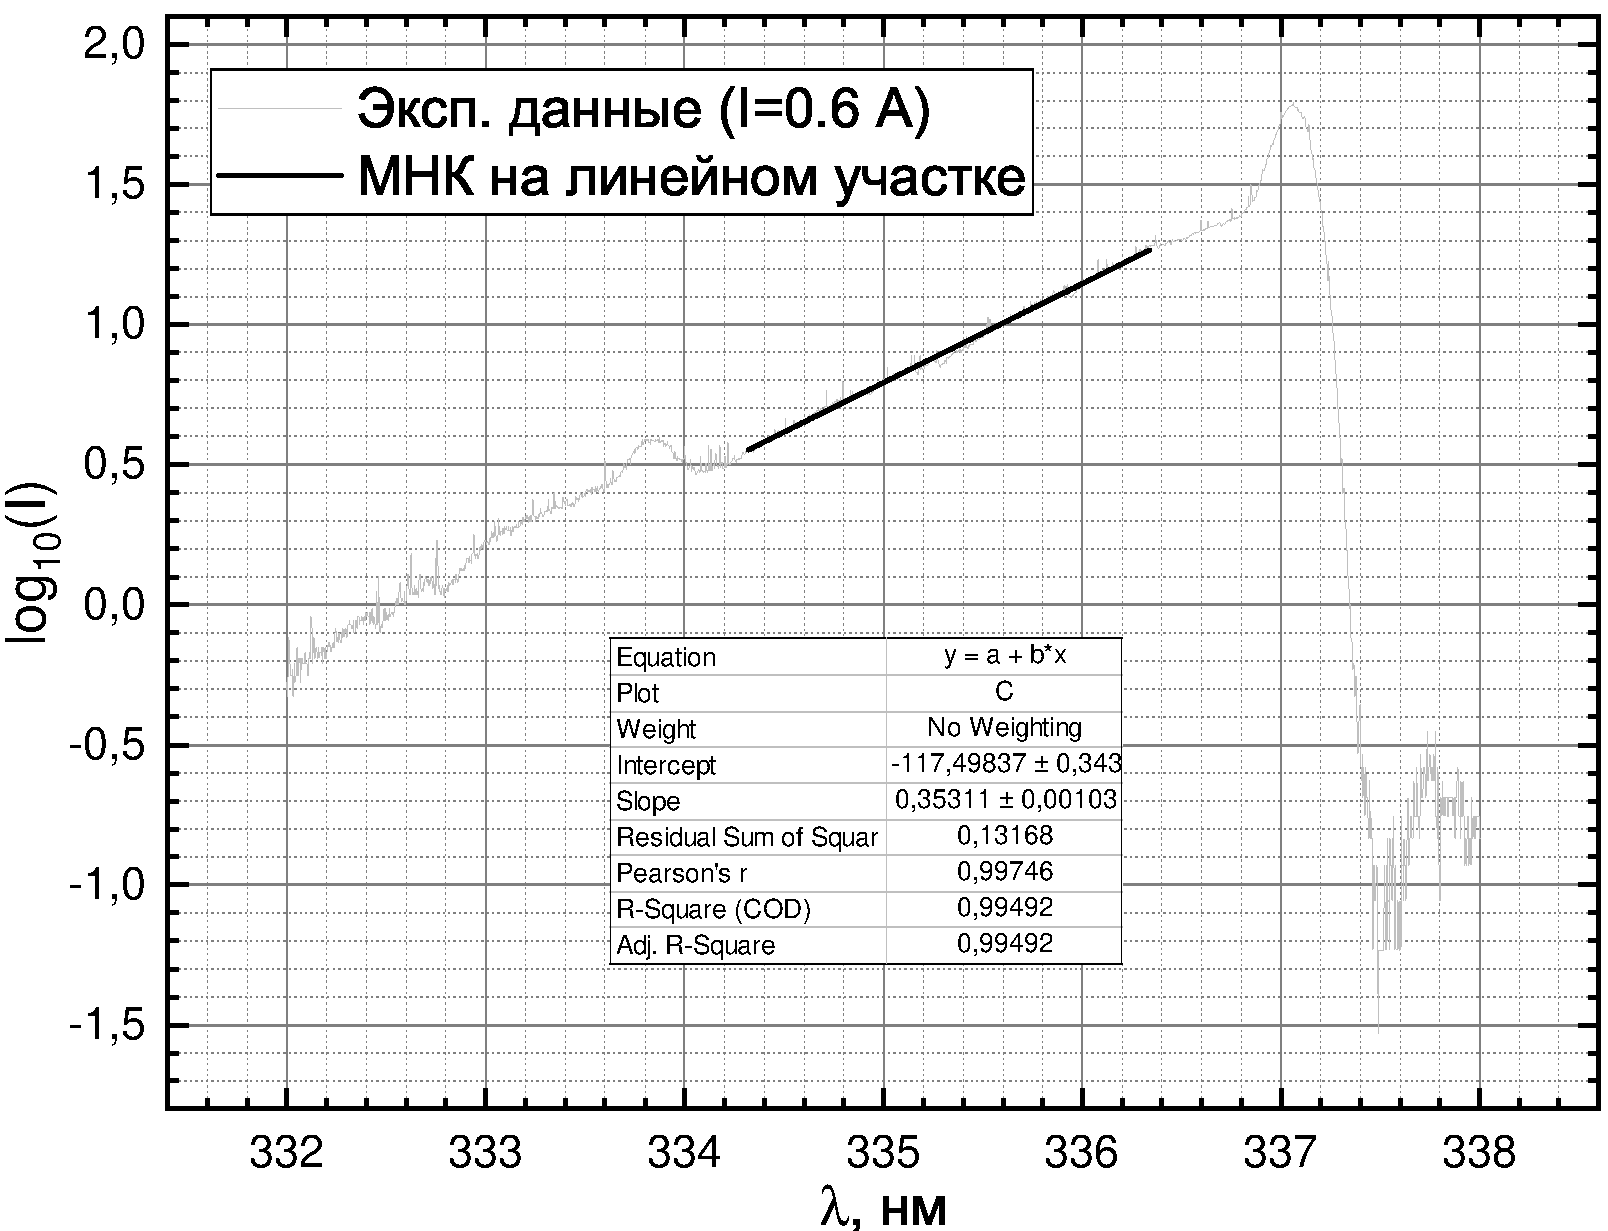
\includegraphics[width=\linewidth]{data/graph_I=0,60_polosa}
		\caption{Спектр при $I= 0.60 $ А, $P$= 36.5 торр}
		\label{polosa_60}
	\end{minipage}
	\begin{minipage}{0.45\linewidth}
		\centering
		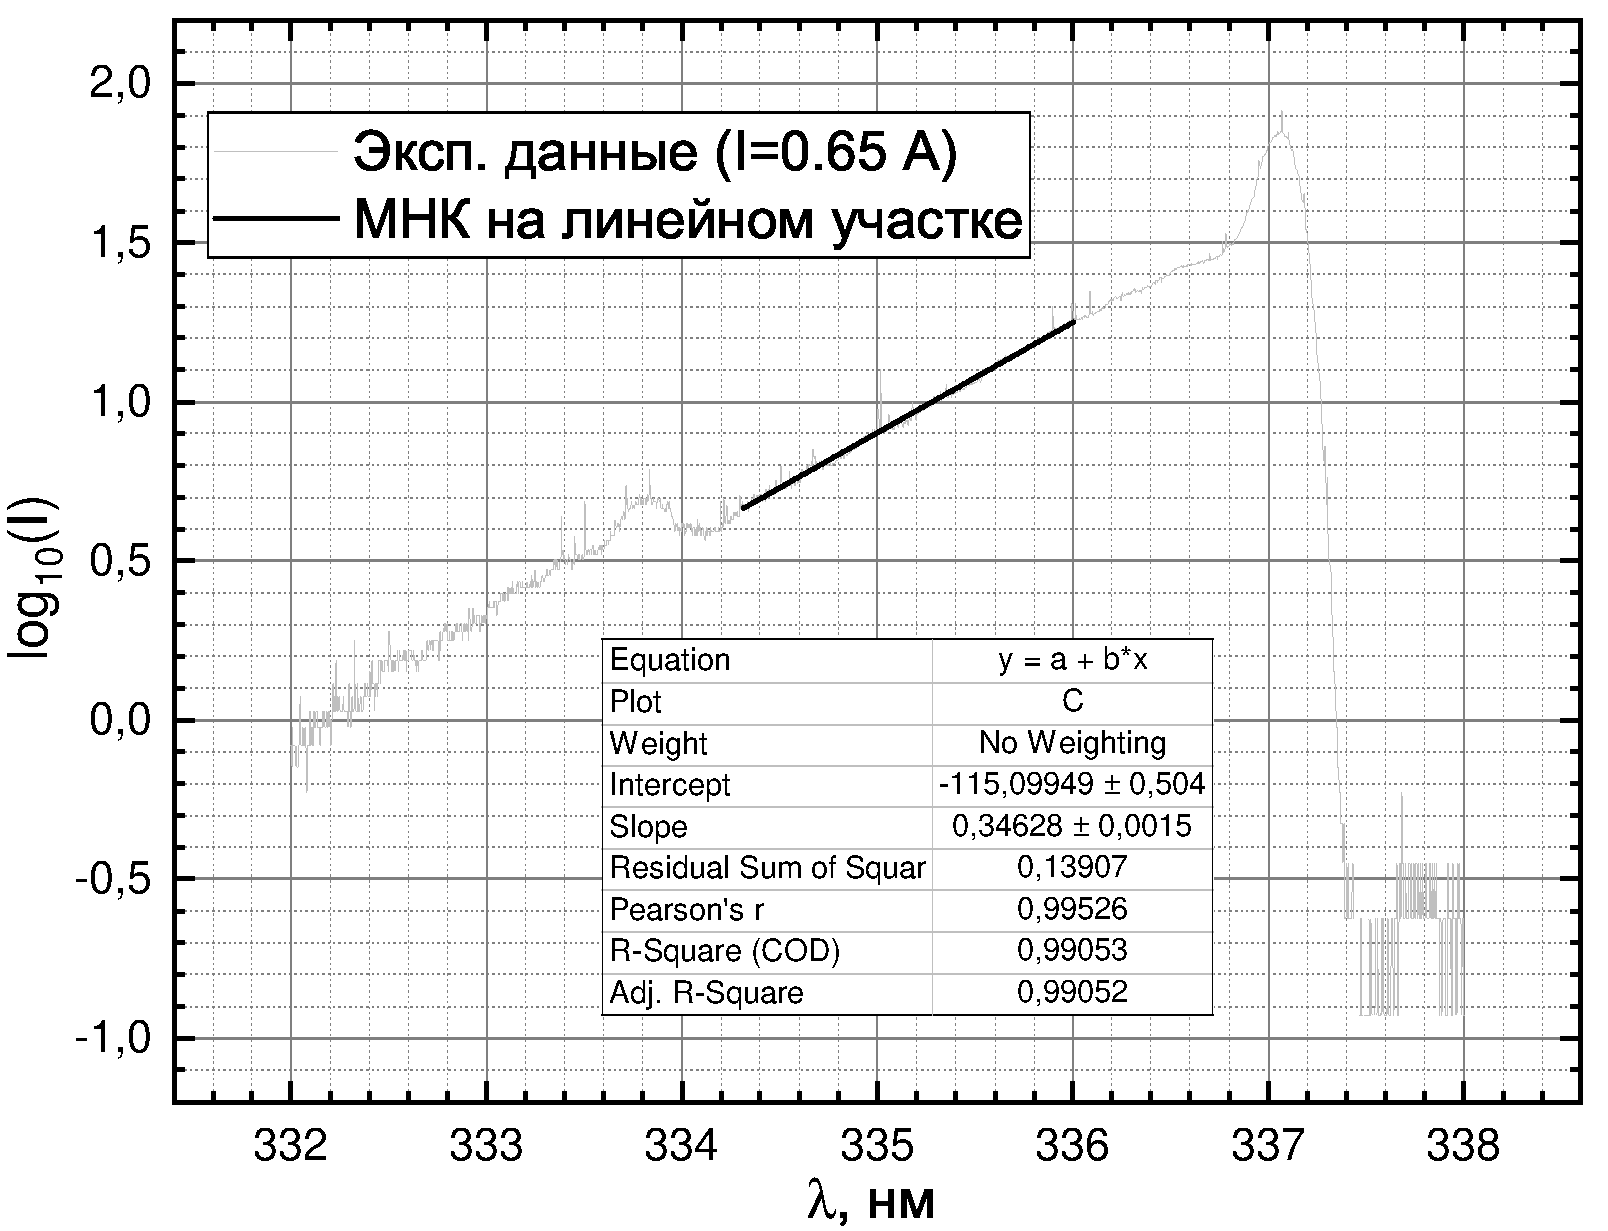
\includegraphics[width=\linewidth]{data/graph_I=0,65_polosa}
		\caption{Спектр при $I= 0.65 $ А, $P$= 36.5 торр}	
		\label{polosa_65}
	\end{minipage} 
	\hfill
\end{figure}